\chapter{Model and General Principles}
\label{ch:background}

This chapter will discuss the model and general principles, which serve the foundation to understand the implementation reports of the following chapter. Its important to understand every subsection of this chapter, such as the ethereum blockchain, \ac{PoW}, the \ac{EVM} and all topics needed for atmoic cross-chain swaps. 

% MB NOT HERE - - write about bitcoin and what changes it brought - buterin eth paper

%
% Section: Der erste Abschnitt
%
\section{Ethereum Blockchain}
\label{sec:background:first_section}
The Ethereum blockchain was introduced in Vitalik Buterin’s paper in 2013, which addressed several limitations of the Bitcoin’s scripting language \cite{buterin2013ethereum} based on Buterin's white paper Wood released the yellow paper one year later \cite{wood2014ethereum}. The main contributions are full Turing-completeness and saving all states of computations in between the states \cite{dannen2017introducing}.
Through its own programming language Solidity, it provides an abstract layer enabling anyone to create their own rules for ownership, formats of transactions, and state transition functions \cite{vujivcic2018blockchain}. Development was funded by an online crowdsale that took place between July and August 2014 \cite{tapscott2016blockchain}. The system then went live on 30 July 2015 \footfullcite{"Ethereum Launches" - https://blog.ethereum.org/2015/07/30/ethereum-launches/. Retrieved 30 July 2015} and is called the ethereum public blockchain. Which means its accessible to everyone who wants to send Ether token or execute smart contracts. In general we have to distinguish between private and public blockchains. The public one is described above. Since everybody can go to github and fork e.g the geth client its possible to start an own private blockchain. In an enterprise software context, where corporate stakeholders are given certain rights and privileges to read and write to the company chain, the deployment is known as a permissioned blockchain. Nevertheless for both the private (permissioned) and the public blockchain its possible to do the following \cite{dannen2017introducing}:

\begin{itemize}
	\item Send and receive Ether
	\item Write smart contracts
	\item Create provably fair applications
	\item Launch your own token based on Ether
\end{itemize}

% ADD LINEBREAK TO FOOTNOTE AND ADD THIS AT THE BEGINNING   Foundation, Ethereum 

\clearpage

\subsection{Proof-of-Work Consensus Algorithm}
\label{subsec:background:first_section:second_subsection}

The \ac{PoW} system of bitcoin and etheruem is similar to Adam Back's Hashcash \cite{back2002hashcash}, but instead of a newspaper or Usenet post the \ac{PoW} involves scanning for a value, which is hashed wish \ac{SHA-256} to begin with a number of zero bits. the average work required is exponential, which means the more leading zeros, the more work. the work can be later verified by executing a single hash. the pow is implemented by incrementing a nonce in the block until a value is found that gives the block's hash the required zero bits. The majority decision is represented by the longest chain, which has the greatest \ac{PoW} effort invested in it. Because later blocks are chained after the premature block, he work to change the block would include redoing all the blocks after it. To modify a past block, an attacker would need to redo all the past work until the specific block he wants to change \cite{nakamoto2008peer}. 

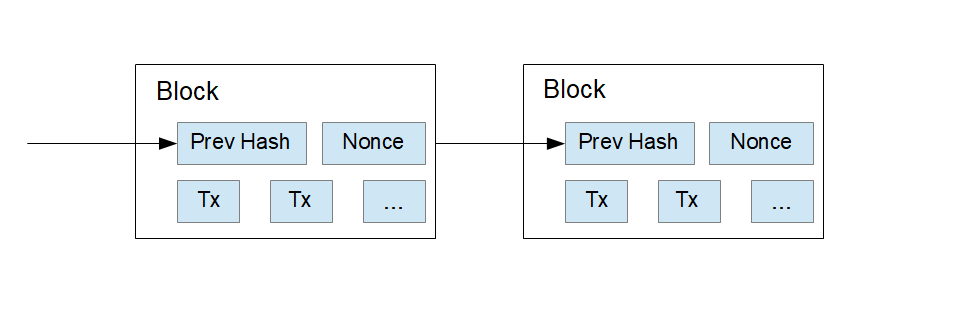
\includegraphics[height=4cm]{blocks}
%ABBILDUNG chapter 4. proof-of-work bitcoin papper nachbauen!!!


%Xiao-Weng Fang: Encyclopedia of Cryptography and Security, Band 1: Computational Puzzles. 2. Auflage. Springer, 2011, ISBN 978-1-4419-5905-8, S. 244 f.
\cite{van2014encyclopedia} sha-256

\cite{isoSHA-256} iso sha became standard 2003 %https://www.iso.org/standard/67116.html
\cite{coron2005merkle} all sha functions start by padding the mnessage according to the so called merkle darmgard strenthenign technique


\subsection{Ethereum Virtual Machine}
\label{subsec:background:first_section:ethereum}
EXPLAIN ETHEREUM \ac{EVM}

\cite{dannen2017introducing}
	%read the evm page 47
%ref to eth paper
\cite{wood2014ethereum}

\subsection{Smart Contracts}
\label{subsec:background:first_section:first_subsection}
EXPLAIN SMART CONTRACTS HERE 
in ethereum context by wood known simple as contracts
buterin first introduced the term smart contracts
% https://cryptorating.eu/whitepapers/Ethereum/Ethereum_white_paper.pdf
\cite{buterin2013ethereum}
% https://files.gitter.im/ethereum/yellowpaper/VIyt/Paper.pdf
\cite{wood2014ethereum}
% https://solidity.readthedocs.io/en/v0.4.24/introduction-to-smart-contracts.html
% https://link.springer.com/content/pdf/bfm%253A978-1-4842-2535-6%252F1.pdf
\cite{dannen2017introducing}



%\subsection{Assets / Cryptocurrencies (Terminology!!)}
%\label{subsec:background:first_section:third_subsection}
%EXPLAIN ASSETS/CRYPTOS HERE

%\subsection{Public and Private Key (Terminology!!)}
%\label{subsec:background:first_section:fourth_subsection}
%EXPLAIN PUBLIC AND PRIVATE KEYS HERE

%
% Section: Der Zweite Abschnitt
%
\section{Digraphs}
\label{sec:background:second_section}
EXPLAIN DIGRAPHS HERE
\cite{bang2007theory}

\section{Hashlocks and Timelocks}
\label{sec:background:third_section}
EXPLAIN HASH AND TIMELOCKS HERE

%\section{Atomic Transactions (Terminology!!)}
%\label{sec:background:fourth_section}
%EXPLAIN ATOMIC TRANSACTIONS HERE

\section{Atomic Cross-Chain Swaps}
\label{sec:background:fifth_section}

theres also research specifically for ethereum private sidechains \cite{robinson2019atomic}
EXPLAIN ATOMIC CROSS CHAIN SWAPS HERE
\cite{herlihy2018atomic}